\chapter{Análisis de la Competencia}
Para la búsqueda de aplicaciones que sean competencia total y parcial se han usado las herramientas online \href{https://www.slant.co}{Slant} y \href{https://alternativeto.net}{AlternativeTo} que ofrecen distintas alternativas a software pre-existente, además de los buscadores de aplicaciones de Google Play y Apple Store.

\section{Aplicaciones encontradas que son competencia total}
\subsection{My Kitchen}
\begin{wrapfigure}[4]{l}{2cm}
\vspace{-.5cm}
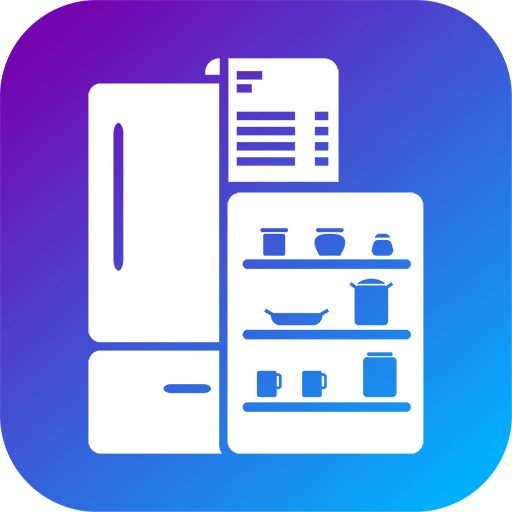
\includegraphics[trim,width=1.8cm]{images/mykitchen.png}
\end{wrapfigure}

La aplicación \href{https://play.google.com/store/apps/details?id=com.peytu.bestbefore}{My Kitchen} está diseñada para reducir el gasto de comida, recordándote qué alimentos de tu cocina van a caducar. Puedes crear un grupo para compartir el inventario con tus compañeros de piso, tu familia o amigos. Para introducir un elemento a tu inventario, puedes hacerlo manualmente o escaneando el código de barras del producto. Las únicas categorías disponibles son basadas en ubicación (Congelador/Nevera/Despensa/Lista de la Compra). Te permite añadir imágenes encontradas con el buscador \href{https://www.ecosia.org/}{Ecosia}, pero no subir tu propia imagen.

De esta aplicación destacamos su interfaz poco accesible y difícil de usar.

\subsection{Best Before: Product Tracker}
\begin{wrapfigure}[4]{r}{2cm}
\flushright
\vspace{-1cm}

\includegraphics[trim,width=1.8cm]{images/bestbefore.png}
\end{wrapfigure}
Sin embargo, \href{https://play.google.com/store/apps/details?id=com.peytu.bestbefore}{Best Before: Product Tracker} está más enfocada a seguir todo el ciclo de vida de un producto, desde que aparece en la lista de la compra, es comprado, abierto (consumido parcialmente), y acabado (o caducado).

Un apartado interesante es el apartado de Consumo, en el que podemos ver qué productos hemos acabado totalmente, y cuales han caducado sin que los hayamos agotado, de esta manera podemos saber qué alimentos suelen caducar y, por lo tanto, deberíamos comprar en menor cantidad. Aunque nos permite guardar el precio de los productos, no hay funcionalidades que lo usen; sería útil usar dicha información para calcular cuanto dinero se «caduca», o si hemos aumentado nuestro consumo de alimentos respecto al mes anterior, etc.

\subsection{Food Checklist}
\begin{wrapfigure}[4]{l}{2cm}
\vspace{-.5cm}
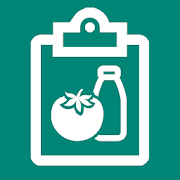
\includegraphics[trim,width=1.8cm]{images/foodchecklist.png}
\end{wrapfigure}
Esta simple aplicación cumple su función. \href{https://play.google.com/store/apps/details?id=com.chestersw.foodlist}{Food Checklist} permite crear varias listas y compartirlas con otras personas. Su diseño sencillo la hace más parecido a una lista de tareas clásica, pero tal vez por eso sea más familiar para el usuario. No tiene categorías ni \textit{espacios} predefinidos, por lo que hay que crearlos a mano.

\section{Aplicaciones encontradas que son competencia parcial}
\subsection{Google Keep}
\begin{wrapfigure}[4]{l}{2cm}
\vspace{-.5cm}

\includegraphics[width=1.8cm]{images/googlekeep.png}
\end{wrapfigure}
Se trata de una simple aplicación de notas con múltiples funcionalidades que hacen que pueda servir para cualquier cosa. Aun así, al ser una simple aplicación de notas, no podemos asignar nada por cada ítem: las propiedades de notificación, categoría, foto, etc. son siempre aplicadas a toda una lista.

\subsection{Listonic}
\begin{wrapfigure}[4]{l}{2cm}
\vspace{-.5cm}

\includegraphics[width=1.8cm]{images/listonic.png}
\end{wrapfigure}
Lista de la compra multiplataforma con multitud de funcionalidades, enfocado en compartirlas con grupos de personas. También es destacable que da diversos consejos sobre compras, ahorro, salud y comidas que hacer con los productos comprados, además de ofrecer tickets descuento de varias compañías. Automáticamente nos calcula el precio de la compra, pero no hay disponible funcionalidades para gestionar los alimentos de los que dispones en casa.

\subsection{Bring}
\begin{wrapfigure}[4]{l}{2cm}
\vspace{-.5cm}

\includegraphics[width=1.8cm]{images/bring.png}
\end{wrapfigure}
Bring está mucho más enfocada a las funcionalidades sociales, puedes tener varias listas, y una foto que identifique la lista del resto. 

Además, puedes saber quien ha añadido un elemento a la lista. Permite enviar mensajes rápidos entre las personas de la lista como «¡Me voy de compras: última oportunidad para añadir cosas a la lista!» o «Compras realizadas». Se sincroniza en tiempo real, por lo que también se puede usar para hacer la compra más rápido entre 2 personas. 

Cuenta con interfaz de voz con el Asistente de Google y Alexa, además de interfaz de Android Wear, no es necesario tan si quiera sacar el móvil mientras estás comprando o si te acuerdas de que hay que comprar algo mientras estás cocinando. 

\section{Tablas de aplicaciones y funcionalidades}
\begin{table}[h]
    \centering
    \begin{threeparttable}
    \rowcolors{3}{white}{black!15}
    \begin{tabular}{@{}rcccccccccccccc@{}}
    \textbf{Aplicación} & 
    \rotatebox{90}{\textbf{Despensa}} &
    \rotatebox{90}{\textbf{Lista de Compra}} &
    \rotatebox{90}{\textbf{Notificaciones}} &
    \rotatebox{90}{\textbf{Caducidad}} &
    \rotatebox{90}{\textbf{Compartir listas}} & 
    \rotatebox{90}{\textbf{Comunicación}} &
    \rotatebox{90}{\textbf{Fotos}} & 
    \rotatebox{90}{\textbf{Precios}} &
    \rotatebox{90}{\textbf{Ubicación}} &
    \rotatebox{90}{\textbf{Categorías}} & 
    \rotatebox{90}{\textbf{Esc. C. Barras}} &
    \rotatebox{90}{\textbf{Esc. Ticket}} &
    \rotatebox{90}{\textbf{Esc. Producto}} &
    \rotatebox{90}{\textbf{Voz}} \\
    \toprule
    \rowcolor{green!30}
    \productname         & \cmark & \cmark & \cmark & \cmark & \cmark & \cmark & \cmark & ? & \cmark & \cmark & ? & ? & ? & ? \\
    \midrule
    My Kitchen           & \cmark & \cmark & \cmark & \cmark & \cmark & \xmark & \zmark\tnote{1} & \xmark & \cmark & \xmark & \cmark & \xmark & \xmark & \xmark \\
    Best Before          & \cmark & \cmark & \cmark & \cmark & \xmark & \xmark & \cmark & \cmark & \cmark & \cmark & \cmark & \xmark & \xmark & \xmark  \\
    Food Checklist       & \cmark & \cmark & \cmark & \cmark & \cmark\tnote{2} & \xmark & \cmark\tnote{2} & \cmark & \cmark & \cmark & \cmark & \xmark & \xmark & \xmark \\
    \midrule
    Google Keep          & \zmark & \zmark & \cmark & \xmark & \cmark & \xmark & \zmark\tnote{3} & \xmark & \xmark & \xmark & \xmark & \xmark & \xmark & \cmark \\
    Listonic             & \xmark & \cmark & \xmark & \xmark & \cmark & \xmark & \cmark & \cmark & \xmark & \cmark & \xmark & \xmark & \xmark & \xmark \\
    Out of Milk          & \xmark & \cmark & \cmark & \xmark & \cmark & \cmark & \cmark & \cmark & \xmark & \cmark & \xmark & \xmark & \xmark & \cmark \\
    \bottomrule
    \end{tabular}
    \begin{tablenotes}
    \footnotesize
    \item[1] Sólo en Ecosia (no se pueden subir fotos propias)
    \item[2] Sólo versión premium
    \item[3] Sólo una foto por nota (lista)
    \end{tablenotes}
    \end{threeparttable}
\end{table}
